% =============================================================================
%  SpikingResNetClassifier Architecture Diagram
%  SWEEP-Net: Spiking Weakly-supervised EEG Emotion Prototyping Network
%  
%  Compile: pdflatex architecture_classifier.tex
% =============================================================================
\documentclass[border=12pt]{standalone}
\usepackage{tikz}
\usepackage{amsmath,amssymb}
\usepackage[T1]{fontenc}
\usepackage{lmodern}

\usetikzlibrary{
  positioning,
  arrows.meta,
  fit,
  calc,
  decorations.pathreplacing,
  backgrounds,
  shapes.geometric
}

% ==============================
%  Color Palette
% ==============================
\definecolor{inputcol}{HTML}{B0BEC5}   % Gray-blue
\definecolor{stemcol}{HTML}{FFCC80}    % Warm orange
\definecolor{convcol}{HTML}{64B5F6}    % Blue
\definecolor{spikecol}{HTML}{81C784}   % Green
\definecolor{tsmcol}{HTML}{CE93D8}     % Purple
\definecolor{poolcol}{HTML}{4DD0E1}    % Cyan
\definecolor{projcol}{HTML}{7986CB}    % Indigo
\definecolor{addcol}{HTML}{FFD54F}     % Amber
\definecolor{dropcol}{HTML}{B0BEC5}    % Gray
\definecolor{normcol}{HTML}{FFB74D}    % Orange
\definecolor{skipcol}{HTML}{EF9A9A}    % Red-pink
\definecolor{identcol}{HTML}{E0E0E0}   % Light gray

% ==============================
%  3D Feature Map Block
% ==============================
%  #1 = name   #2 = left-x   #3 = fill color
%  #4 = height (spatial)  #5 = width  #6 = z-depth (channels)
\newcommand{\featBlock}[6]{%
  % --- Front face ---
  \fill[#3!50!white, draw=#3!30!black, line width=0.6pt]
    ({#2}, {-(#4)/2}) rectangle ({#2+(#5)}, {(#4)/2});
  % --- Right side face ---
  \fill[#3!70!white, draw=#3!30!black, line width=0.5pt]
    ({#2+(#5)}, {-(#4)/2}) -- 
    ({#2+(#5)+(#6)}, {-(#4)/2+(#6)}) -- 
    ({#2+(#5)+(#6)}, {(#4)/2+(#6)}) -- 
    ({#2+(#5)}, {(#4)/2}) -- cycle;
  % --- Top face ---
  \fill[#3!35!white, draw=#3!30!black, line width=0.5pt]
    ({#2}, {(#4)/2}) -- 
    ({#2+(#6)}, {(#4)/2+(#6)}) -- 
    ({#2+(#5)+(#6)}, {(#4)/2+(#6)}) -- 
    ({#2+(#5)}, {(#4)/2}) -- cycle;
  % --- Connection coordinates ---
  \coordinate (#1-east) at ({#2+(#5)+(#6)}, 0);
  \coordinate (#1-west) at ({#2}, 0);
  \coordinate (#1-south) at ({#2+(#5)/2}, {-(#4)/2});
  \coordinate (#1-top) at ({#2+(#5)/2+(#6)/2}, {(#4)/2+(#6)/2});
  \coordinate (#1-center) at ({#2+(#5)/2+(#6)/2}, {(#6)/2});
}

\begin{document}
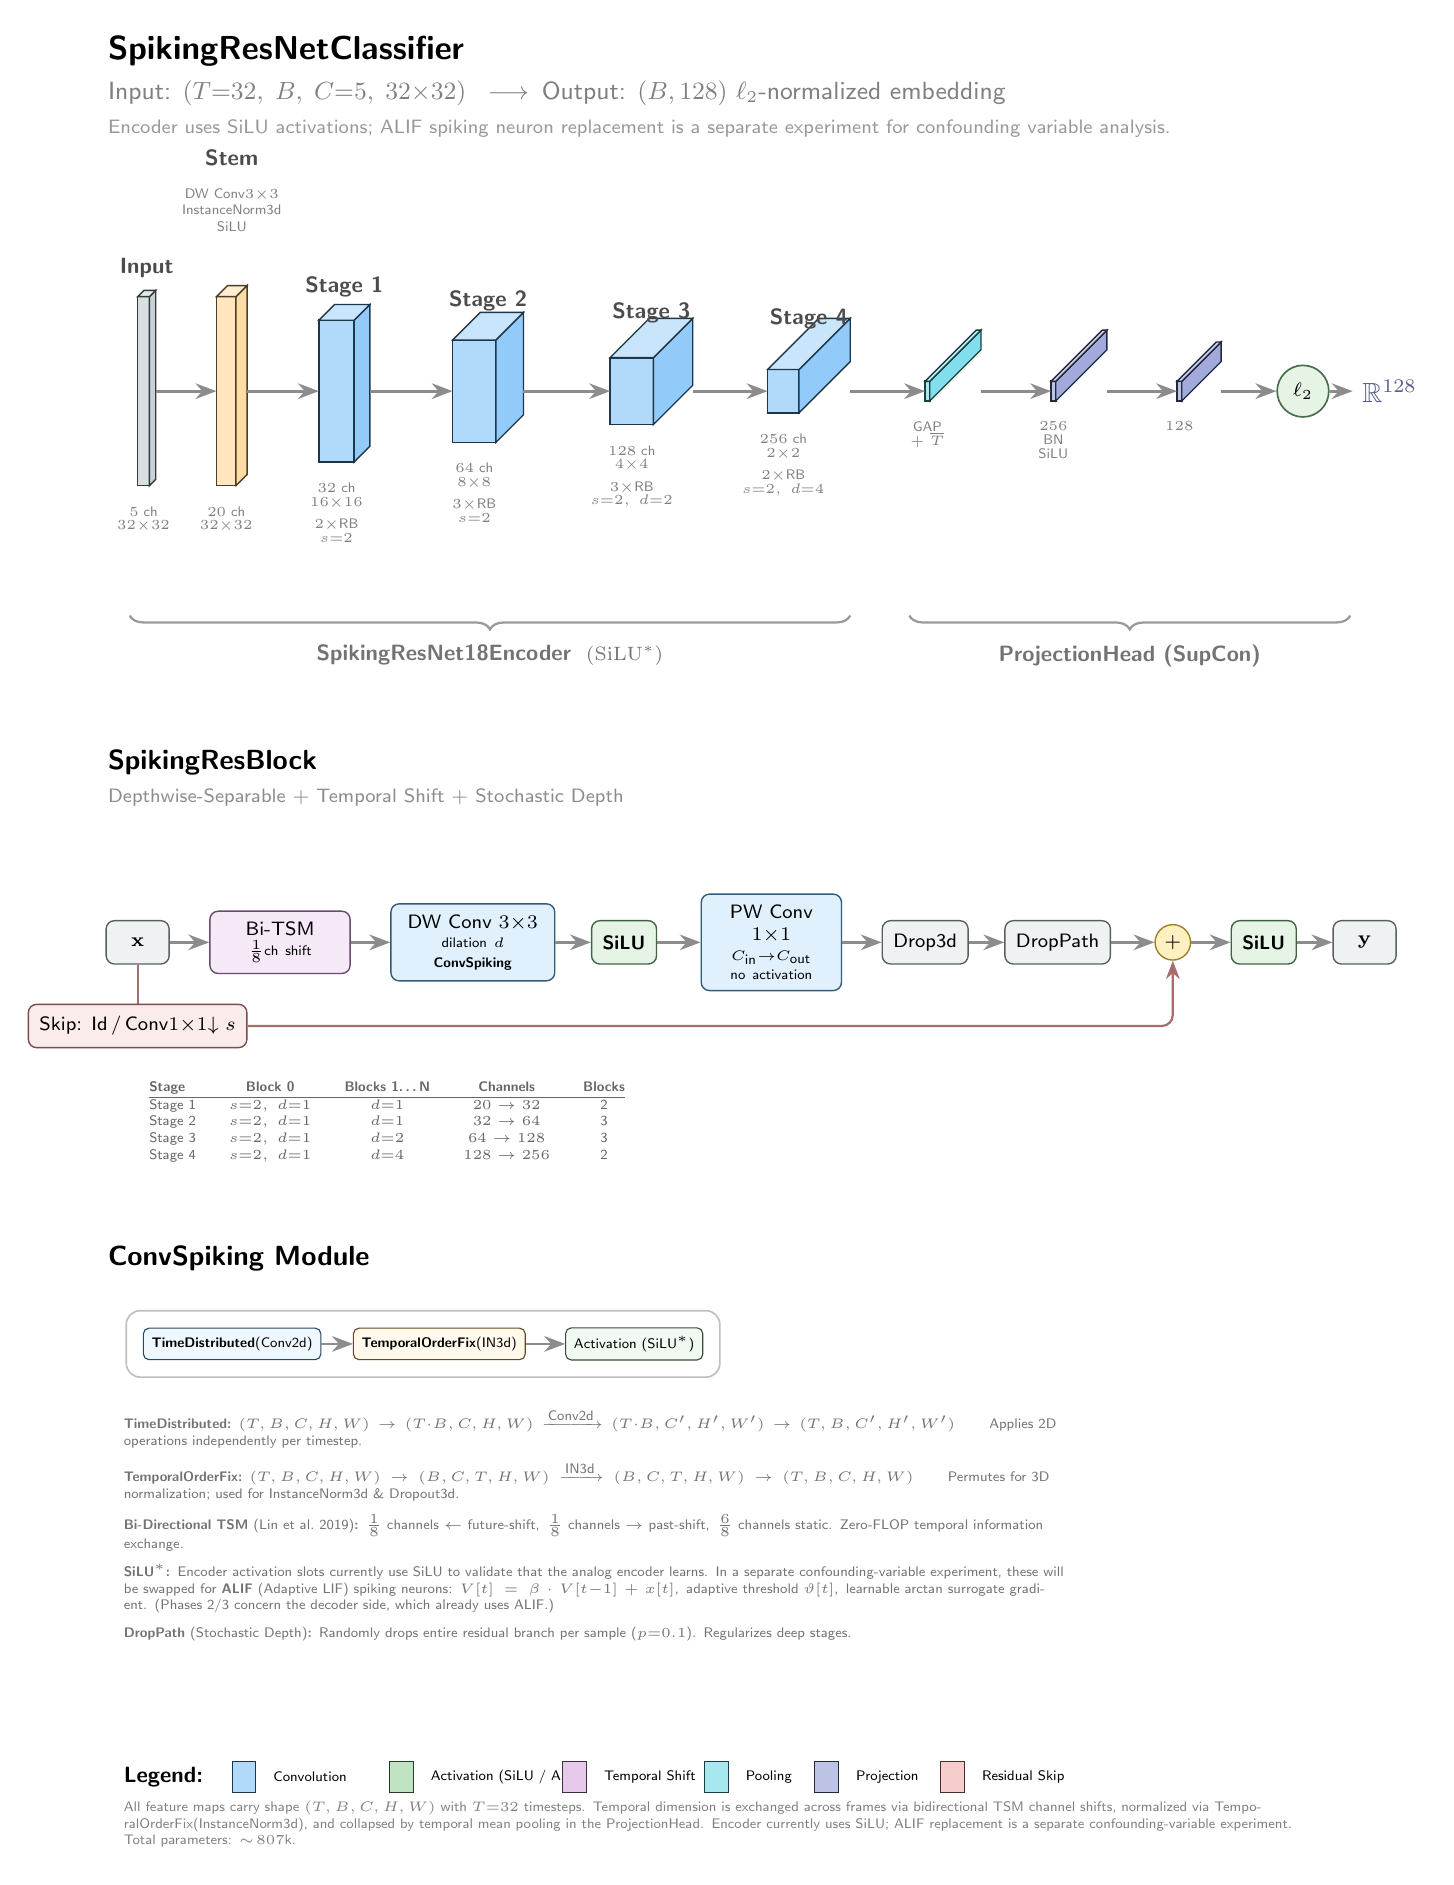
\begin{tikzpicture}[
  >=Stealth,
  font=\sffamily\small,
  % Arrow style
  arrow/.style={->, line width=1pt, draw=black!45},
  % Label styles
  lbl/.style={font=\scriptsize\sffamily, align=center, text=black!80},
  stglbl/.style={font=\footnotesize\sffamily\bfseries, text=black!70},
  dimlbl/.style={font=\tiny\sffamily, text=black!50, align=center},
  % Flowchart node styles
  opbox/.style n args={1}{
    draw=#1!50!black, fill=#1!20!white,
    rounded corners=3pt, minimum height=0.55cm,
    font=\scriptsize\sffamily, inner sep=4pt, line width=0.5pt
  },
  addnode/.style={
    circle, draw=addcol!60!black, fill=addcol!35!white,
    minimum size=0.45cm, font=\scriptsize\bfseries, inner sep=0pt,
    line width=0.5pt
  },
  detailbox/.style={
    draw=black!25, fill=white, rounded corners=5pt,
    inner sep=8pt, line width=0.6pt
  },
  modulebox/.style n args={1}{
    draw=#1!40!black, fill=#1!10!white, rounded corners=2pt,
    font=\tiny\sffamily, inner sep=3pt, minimum height=0.4cm
  },
]

% =====================================================================
%  PART 1: MAIN PIPELINE (3D blocks)
% =====================================================================

% --- Title ---
\node[font=\large\sffamily\bfseries, anchor=south west] at (-0.5, 4.0)
  {SpikingResNetClassifier};
\node[font=\small\sffamily, text=black!50, anchor=south west] at (-0.5, 3.5)
  {Input: $(T{=}32,\; B,\; C{=}5,\; 32{\times}32)$ \enspace$\longrightarrow$\enspace 
   Output: $(B, 128)$ $\ell_2$-normalized embedding};
\node[font=\scriptsize\sffamily, text=black!40, anchor=south west] at (-0.5, 3.1)
  {Encoder uses SiLU activations; ALIF spiking neuron replacement is a separate experiment for confounding variable analysis.};

% --- 3D Feature Blocks ---
% featBlock{name}{left-x}{color}{height}{width}{z-depth}

% Input (5 channels, 32x32)
\featBlock{input}{0.0}{inputcol}{2.4}{0.15}{0.08}

% Stem (20 channels, 32x32)
\featBlock{stem}{1.0}{stemcol}{2.4}{0.25}{0.14}

% Stage 1 (32 channels, 16x16)
\featBlock{s1}{2.3}{convcol}{1.8}{0.45}{0.20}

% Stage 2 (64 channels, 8x8)
\featBlock{s2}{4.0}{convcol}{1.3}{0.55}{0.35}

% Stage 3 (128 channels, 4x4)
\featBlock{s3}{6.0}{convcol}{0.85}{0.55}{0.50}

% Stage 4 (256 channels, 2x2)
\featBlock{s4}{8.0}{convcol}{0.55}{0.40}{0.65}

% GAP + Temporal Mean (256 channels, 1x1)
\featBlock{gap}{10.0}{poolcol}{0.25}{0.06}{0.65}

% FC1: Conv1x1 256->256 + BN + SiLU
\featBlock{fc1}{11.6}{projcol}{0.25}{0.06}{0.65}

% FC2: Conv1x1 256->128
\featBlock{fc2}{13.2}{projcol}{0.25}{0.06}{0.50}

% L2 Normalize
\node[circle, draw=spikecol!55!black, fill=spikecol!20!white,
      minimum size=0.55cm, line width=0.6pt, font=\scriptsize\bfseries]
  (l2) at (14.8, 0) {$\ell_2$};

% Output embedding
\node[font=\normalsize\sffamily\bfseries, text=projcol!70!black] 
  (emb) at (15.9, 0) {$\mathbb{R}^{128}$};

% --- Arrows between blocks ---
\draw[arrow] (input-east) -- (stem-west);
\draw[arrow] (stem-east) -- (s1-west);
\draw[arrow] (s1-east) -- (s2-west);
\draw[arrow] (s2-east) -- (s3-west);
\draw[arrow] (s3-east) -- (s4-west);
\draw[arrow] (s4-east) -- (gap-west);
\draw[arrow] (gap-east) -- (fc1-west);
\draw[arrow] (fc1-east) -- (fc2-west);
\draw[arrow] (fc2-east) -- (l2.west);
\draw[arrow] (l2.east) -- (emb.west);

% --- Stage labels (above blocks) ---
\node[stglbl] at (input-top) [above=2pt] {Input};
\node[stglbl] at (stem-top) [above=42pt] {Stem};
\node[stglbl] at (s1-top) [above=2pt] {Stage 1};
\node[stglbl] at (s2-top) [above=2pt] {Stage 2};
\node[stglbl] at (s3-top) [above=2pt] {Stage 3};
\node[stglbl] at (s4-top) [above=2pt] {Stage 4};

% --- Dimension labels (below blocks) ---
\node[dimlbl] at (input-south) [below=4pt] {$5$ ch\\[-1pt]$32{\times}32$};

\node[dimlbl] at (stem-south) [below=4pt]
  {$20$ ch\\[-1pt]$32{\times}32$};

\node[dimlbl] at (s1-south) [below=4pt]
  {$32$ ch\\[-1pt]$16{\times}16$\\[2pt]\tiny$2{\times}$RB\\[-1pt]\tiny$s{=}2$};

\node[dimlbl] at (s2-south) [below=4pt]
  {$64$ ch\\[-1pt]$8{\times}8$\\[2pt]\tiny$3{\times}$RB\\[-1pt]\tiny$s{=}2$};

\node[dimlbl] at (s3-south) [below=4pt]
  {$128$ ch\\[-1pt]$4{\times}4$\\[2pt]\tiny$3{\times}$RB\\[-1pt]\tiny$s{=}2,\;d{=}2$};

\node[dimlbl] at (s4-south) [below=4pt]
  {$256$ ch\\[-1pt]$2{\times}2$\\[2pt]\tiny$2{\times}$RB\\[-1pt]\tiny$s{=}2,\;d{=}4$};

\node[dimlbl] at (gap-south) [below=4pt]
  {GAP\\[-1pt]$+\;\overline{T}$};

\node[dimlbl] at (fc1-south) [below=4pt]
  {$256$\\[-1pt]BN\\[-1pt]SiLU};

\node[dimlbl] at (fc2-south) [below=4pt]
  {$128$};

% --- Encoder / Projection braces ---
\draw[decorate, decoration={brace, amplitude=5pt, mirror}, thick, draw=black!40]
  (-0.1, -2.85) -- (9.05, -2.85)
  node[midway, below=7pt, font=\footnotesize\sffamily\bfseries, text=black!55]
  {SpikingResNet18Encoder \;{\normalfont\scriptsize(SiLU$^*$)}};

\draw[decorate, decoration={brace, amplitude=5pt, mirror}, thick, draw=black!40]
  (9.8, -2.85) -- (15.4, -2.85)
  node[midway, below=7pt, font=\footnotesize\sffamily\bfseries, text=black!55]
  {ProjectionHead (SupCon)};

% --- Stem detail annotation (above the block) ---
\node[dimlbl, anchor=south, text width=2.2cm] at (stem-top) [above=18pt]
  {DW Conv$3{\times}3$\\InstanceNorm3d\\SiLU};


% =====================================================================
%  PART 2: SpikingResBlock (Detailed Internal View)
% =====================================================================

\begin{scope}[yshift=-7.0cm]

\node[font=\normalsize\sffamily\bfseries, anchor=south west] at (-0.5, 2.0)
  {SpikingResBlock};
\node[font=\scriptsize\sffamily, text=black!45, anchor=south west] at (-0.5, 1.60)
  {Depthwise-Separable $+$ Temporal Shift $+$ Stochastic Depth};

% --- Input ---
\node[opbox={inputcol}, minimum width=0.8cm] (rb-in) at (0, 0) {$\mathbf{x}$};

% --- TSM ---
\node[opbox={tsmcol}, right=0.5cm of rb-in, text width=1.5cm, align=center] (tsm)
  {Bi-TSM\\[-1pt]{\tiny$\frac{1}{8}$ch shift}};

% --- DWConv (ConvSpiking block 1) ---
\node[opbox={convcol}, right=0.5cm of tsm, text width=1.8cm, align=center] (dw)
  {DW Conv $3{\times}3$\\[-1pt]{\tiny dilation $d$}\\[-1pt]{\tiny \textbf{ConvSpiking}}};

% --- SiLU activation after DWConv ---
\node[opbox={spikecol}, right=0.45cm of dw, minimum width=0.8cm] (alif1) 
  {\textbf{SiLU}};

% --- PWConv (ConvSpiking block 2, no activation) ---
\node[opbox={convcol}, right=0.55cm of alif1, text width=1.5cm, align=center] (pw)
  {PW Conv $1{\times}1$\\[-1pt]{\tiny $C_\text{in}{\to}C_\text{out}$}\\[-1pt]{\tiny no activation}};

% --- Dropout ---
\node[opbox={dropcol}, right=0.5cm of pw, minimum width=0.8cm] (drop)
  {Drop3d};

% --- DropPath ---
\node[opbox={dropcol}, right=0.45cm of drop, minimum width=0.9cm] (dpath)
  {DropPath};

% --- Add node ---
\node[addnode, right=0.55cm of dpath] (add) {$+$};

% --- Final SiLU ---
\node[opbox={spikecol}, right=0.5cm of add, minimum width=0.8cm] (alif2)
  {\textbf{SiLU}};

% --- Output ---
\node[opbox={inputcol}, right=0.45cm of alif2, minimum width=0.8cm] (rb-out)
  {$\mathbf{y}$};

% --- Main flow arrows ---
\draw[arrow] (rb-in) -- (tsm);
\draw[arrow] (tsm) -- (dw);
\draw[arrow] (dw) -- (alif1);
\draw[arrow] (alif1) -- (pw);
\draw[arrow] (pw) -- (drop);
\draw[arrow] (drop) -- (dpath);
\draw[arrow] (dpath) -- (add);
\draw[arrow] (add) -- (alif2);
\draw[arrow] (alif2) -- (rb-out);

% --- Skip / Residual connection ---
\draw[line width=0.8pt, draw=skipcol!70!black, rounded corners=4pt, ->]
  (rb-in.south) -- ++(0, -0.9)
  node[pos=0.55, opbox={skipcol}, minimum width=2.2cm, anchor=north]
    (skip) {Skip: Id\,/\,Conv$1{\times}1${\scriptsize$\downarrow s$}}
  ;
\draw[line width=0.8pt, draw=skipcol!70!black, rounded corners=4pt, ->]
  (skip.east) -| (add.south);

% --- Stage configuration table ---
\node[anchor=north west, font=\tiny\sffamily, text=black!60, align=left,
      inner sep=4pt] at (0, -1.6) {%
\begin{tabular}{@{}l c c c c@{}}
  \textbf{Stage} & \textbf{Block 0} & \textbf{Blocks 1\ldots N} & \textbf{Channels} & \textbf{Blocks}\\
  \hline
  Stage 1 & $s{=}2,\; d{=}1$ & $d{=}1$ & $20 \to 32$ & 2 \\
  Stage 2 & $s{=}2,\; d{=}1$ & $d{=}1$ & $32 \to 64$ & 3 \\
  Stage 3 & $s{=}2,\; d{=}1$ & $d{=}2$ & $64 \to 128$ & 3 \\
  Stage 4 & $s{=}2,\; d{=}1$ & $d{=}4$ & $128 \to 256$ & 2 \\
\end{tabular}};

\end{scope}


% =====================================================================
%  PART 3: ConvSpiking Module & Key Components
% =====================================================================

\begin{scope}[yshift=-12.5cm]

\node[font=\normalsize\sffamily\bfseries, anchor=south west] at (-0.5, 1.2)
  {ConvSpiking Module};

% --- ConvSpiking detail ---
\node[modulebox={convcol}] (td) at (1.2, 0.4)
  {\textbf{TimeDistributed}(Conv2d)};
\node[modulebox={normcol}, right=0.4cm of td] (tof)
  {\textbf{TemporalOrderFix}(IN3d)};
\node[modulebox={spikecol}, right=0.5cm of tof] (spike)
  {Activation (SiLU$^*$)};

\draw[arrow] (td) -- (tof);
\draw[arrow] (tof) -- (spike);

% Surrounding box
\begin{scope}[on background layer]
  \node[detailbox, fit=(td)(tof)(spike), inner sep=6pt] (csbox) {};
\end{scope}

% --- Module Descriptions ---
\node[anchor=north west, font=\tiny\sffamily, text=black!55, 
      text width=12cm, align=left] at (-0.3, -0.3) {%
\textbf{TimeDistributed:}\enspace 
$(T,B,C,H,W) \to (T{\cdot}B, C, H, W) \xrightarrow{\text{Conv2d}} 
(T{\cdot}B, C', H', W') \to (T, B, C', H', W')$
\qquad Applies 2D operations independently per timestep.\\[4pt]
\textbf{TemporalOrderFix:}\enspace 
$(T,B,C,H,W) \to (B,C,T,H,W) \xrightarrow{\text{IN3d}} 
(B,C,T,H,W) \to (T,B,C,H,W)$
\qquad Permutes for 3D normalization; used for InstanceNorm3d \& Dropout3d.\\[4pt]
\textbf{Bi-Directional TSM} (Lin et al.~2019)\textbf{:}\enspace 
$\frac{1}{8}$ channels $\leftarrow$ future-shift,\enspace
$\frac{1}{8}$ channels $\rightarrow$ past-shift,\enspace
$\frac{6}{8}$ channels static.\enspace
Zero-FLOP temporal information exchange.\\[4pt]
\textbf{SiLU$^*$:}\enspace 
Encoder activation slots currently use SiLU to validate that the analog encoder learns.\enspace
In a separate confounding-variable experiment, these will be swapped for \textbf{ALIF} (Adaptive LIF) spiking neurons:\enspace
$V[t] = \beta \cdot V[t{-}1] + x[t]$,\enspace
adaptive threshold $\vartheta[t]$,\enspace
learnable arctan surrogate gradient.\enspace
(Phases~2/3 concern the decoder side, which already uses ALIF.)\\[4pt]
\textbf{DropPath} (Stochastic Depth)\textbf{:}\enspace
Randomly drops entire residual branch per sample ($p{=}0.1$).
Regularizes deep stages.
};

\end{scope}


% =====================================================================
%  PART 4: Legend
% =====================================================================

\begin{scope}[yshift=-18.0cm]

\node[font=\footnotesize\sffamily\bfseries, anchor=west] at (-0.3, 0.4) {Legend:};

% Color swatches
\fill[convcol!50!white, draw=convcol!30!black, line width=0.4pt]
  (1.2, 0.2) rectangle (1.5, 0.6);
\node[font=\tiny\sffamily, anchor=west] at (1.6, 0.4) {Convolution};

\fill[spikecol!50!white, draw=spikecol!30!black, line width=0.4pt]
  (3.2, 0.2) rectangle (3.5, 0.6);
\node[font=\tiny\sffamily, anchor=west] at (3.6, 0.4) {Activation (SiLU / ALIF)};

\fill[tsmcol!50!white, draw=tsmcol!30!black, line width=0.4pt]
  (5.4, 0.2) rectangle (5.7, 0.6);
\node[font=\tiny\sffamily, anchor=west] at (5.8, 0.4) {Temporal Shift};

\fill[poolcol!50!white, draw=poolcol!30!black, line width=0.4pt]
  (7.2, 0.2) rectangle (7.5, 0.6);
\node[font=\tiny\sffamily, anchor=west] at (7.6, 0.4) {Pooling};

\fill[projcol!50!white, draw=projcol!30!black, line width=0.4pt]
  (8.6, 0.2) rectangle (8.9, 0.6);
\node[font=\tiny\sffamily, anchor=west] at (9.0, 0.4) {Projection};

\fill[skipcol!50!white, draw=skipcol!30!black, line width=0.4pt]
  (10.2, 0.2) rectangle (10.5, 0.6);
\node[font=\tiny\sffamily, anchor=west] at (10.6, 0.4) {Residual Skip};

% Note about temporal dimension
\node[font=\tiny\sffamily, text=black!50, anchor=west, text width=15cm] at (-0.3, -0.2) 
  {All feature maps carry shape $(T, B, C, H, W)$ with $T{=}32$ timesteps. 
   Temporal dimension is exchanged across frames via bidirectional TSM channel shifts, 
   normalized via TemporalOrderFix(InstanceNorm3d), and collapsed by temporal mean pooling in the ProjectionHead.
   Encoder currently uses SiLU; ALIF replacement is a separate confounding-variable experiment.
   Total parameters: $\sim\!807$k.};

\end{scope}

\end{tikzpicture}
\end{document}
